\documentclass[12pt]{scrartcl}
\input{../styles/Packages.tex}
\input{../styles/FormatAndHeader.tex}
\usepackage{graphicx}

\setcounter{sheetnr}{8} % Nummer des Übungsblattes
\setcounter{exnum}{1} % Nummer der Aufgabe

% Beginn des eigentlichen Dokuments

\begin{document}

% Aufgabe 1
\exercise{Dijkstra-Algorithmus}
\begin{enumerate}
  \item Tabelle
  \begin{center}
    \begin{tabular}{ |c|c|c|c|c|c|c|c| } 
     \hline
     Schritt & A & B & C & D & E & F & G\\ \hline
     1 & $\infty$ & $\infty$ & $\infty$ & $\infty$ & $\infty$ & 0 & $\infty$ \\ \hline
     2 & $\infty$ & 4 & $\infty$ & 5 & $\infty$ & 0 & 1 \\ \hline
     3 & $\infty$ & 3 & $\infty$ & 4 & 8 & 0 & 1 \\ \hline
     4 & $\infty$ & 3 & 5 & 4 & 6 & 0 & 1 \\ \hline
     5 & 9 & 3 & 5 & 4 & 6 & 0 & 1 \\ \hline
     6 & 8 & 3 & 5 & 4 & 6 & 0 & 1 \\ \hline
    \end{tabular}
  \end{center}
  
  \item Beispiel\\
  Vor der Addition ist die kürzeste Pfad von Knoten A zum Knoten C A->B->C.\\
  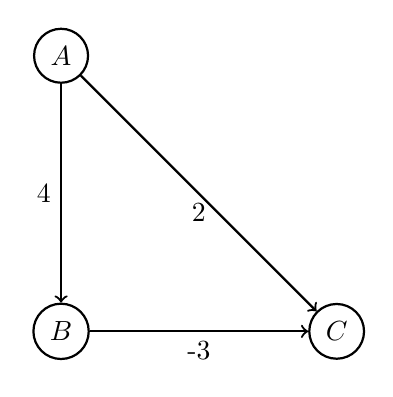
\begin{tikzpicture}[node distance={35mm}, thick, main/.style = {draw, circle}] 
    \node[main] (1) {$A$}; 
    \node[main] (2) [below of=1] {$B$}; 
    \node[main] (3) [right of=2] {$C$}; 
    \draw[->] (1)  -- node[midway, left, pos=0.5] {4} (2) ; 
    \draw[->] (2) -- node[midway, below, pos=0.5] {-3} (3) ;
    \draw[->] (1) -- node[midway, below, pos=0.5] {2} (3) ;
  \end{tikzpicture}
  
  Nach der Addition einer Konstante 4 für jeden Knoten ist die kürzeste Pfad von Knoten A zum Knoten C die Kante A->C mit dem Gewicht 6.\\
  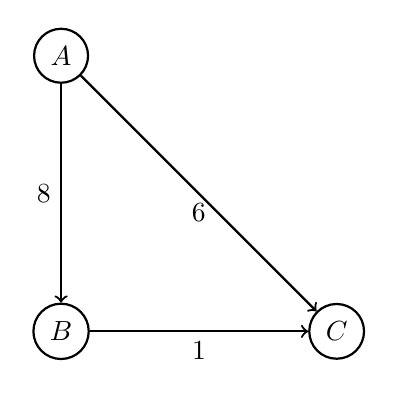
\begin{tikzpicture}[node distance={35mm}, thick, main/.style = {draw, circle}] 
    \node[main] (1) {$A$}; 
    \node[main] (2) [below of=1] {$B$}; 
    \node[main] (3) [right of=2] {$C$}; 
    \draw[->] (1)  -- node[midway, left, pos=0.5] {8} (2) ; 
    \draw[->] (2) -- node[midway, below, pos=0.5] {1} (3) ;
    \draw[->] (1) -- node[midway, below, pos=0.5] {6} (3) ;
  \end{tikzpicture} 

  \item minimaler Spannbaum\\
  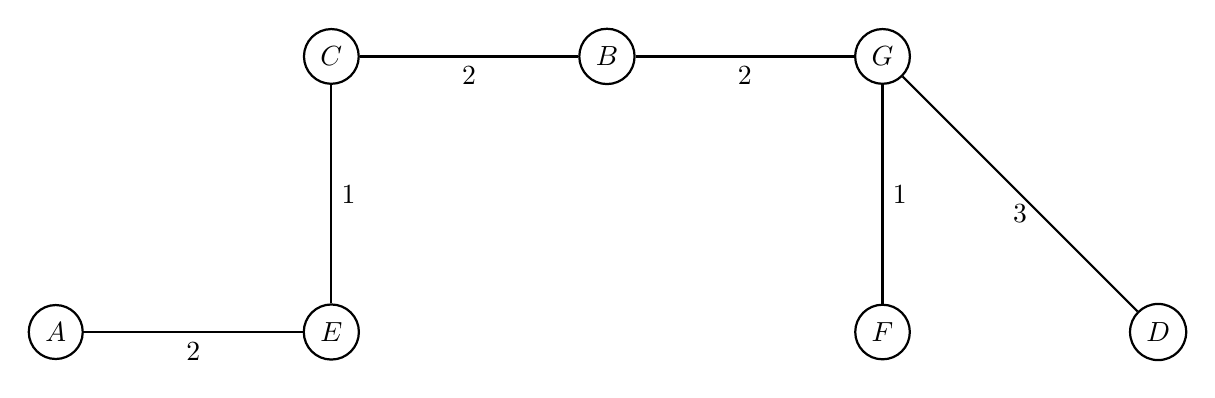
\begin{tikzpicture}[node distance={35mm}, thick, main/.style = {draw, circle}] 
    \node[main] (1) {$A$}; 
    \node[main] (5) [right of=1] {$E$}; 
    \node[main] (3) [above of=5] {$C$}; 
    \node[main] (2) [right of=3] {$B$}; 
    \node[main] (7) [right of=2] {$G$}; 
    \node[main] (6) [below of=7] {$F$}; 
    \node[main] (4) [right of=6] {$D$}; 
    \draw[-] (1)  -- node[midway, below, pos=0.5] {2} (5) ; 
    \draw[-] (5) -- node[midway, right, pos=0.5] {1} (3) ;
    \draw[-] (3) -- node[midway, below, pos=0.5] {2} (2) ;
    \draw[-] (2) -- node[midway, below, pos=0.5] {2} (7) ;
    \draw[-] (7) -- node[midway, right, pos=0.5] {1} (6) ;
    \draw[-] (7) -- node[midway, below, pos=0.5] {3} (4) ;
  \end{tikzpicture} 

\end{enumerate}

\setcounter{exnum}{3} % Nummer der Aufgabe
% Aufgabe 3
\exercise{Delaunary-Triangulierung}
\begin{enumerate}

  \item Plane-Sweep-Algorithmus
  \begin{figure}[!h]
    \centering
      \includegraphics[width=0.5\textwidth]{A3a.png}
    \caption{Plane-Sweep-Algorithmus}
  \end{figure}

  \item Edge-Flip-Algorithmus

  \begin{enumerate}
    \item alle Kanten, die lokalen Delaunary-Eigenschaften verletzt werden.
    \begin{figure}[!h]
      \centering
        \includegraphics[width=0.5\textwidth]{A3b1.png}
      \caption{alle Kanten, die lokalen Delaunary-Eigenschaften verletzt werden}
    \end{figure}

    \newpage
    
    \item Zwischenstände
    \begin{figure}[!h]
      \centering
        \includegraphics[width=0.5\textwidth]{A3b1.png}
      \caption{für die erste Kante}
    \end{figure}
    \begin{figure}[!h]
      \centering
        \includegraphics[width=0.5\textwidth]{A3b2.png}
      \caption{für die zweite Kante}
    \end{figure}

    \newpage

    \item Endzustand
    \begin{figure}[!h]
      \centering
        \includegraphics[width=0.5\textwidth]{A3b3.png}
      \caption{Endzustand}
    \end{figure}
  \end{enumerate}

  \item Begründung: Wenn es insgesamt n Knoten im Graph gibt, gibt es höchstens $n(n-1)/2$ Kanten. Wenn eine Kante bereits für die Triangulierung ausprobiert wird, dabei die 
  lokalen Delaunary-Eigenschaften verletzt werden, wird diese Kante nicht mehr verwendet und ausgewählt. Deswegen terminiert der Algorithmus.
  
\end{enumerate}

\exercise{Multimodales Routing}
\begin{enumerate}
  \item äußere Einflüsse
  \begin{enumerate}
    \item Stau, der passiert oft in einer Großstadt
    \item Wetter, wenn es regnet, wird die Geschwindigkeit dadurch versunken.
    \item Straßenreparatur, sie passiert auch oft in einer Großstadt.
  \end{enumerate}

  \item Für Fußgänger, Verkehrstau kann vernachlässigt werden. Für Personen im Rollstuhl und mit dem E-Scooter kann das Wetter nicht ignoriert werden.
\end{enumerate}

\end{document}
